\documentclass[journal]{IEEEtran}
\usepackage[utf8]{inputenc}
\usepackage[T1]{fontenc}
\usepackage[spanish,es-tabla,es-nodecimaldot,es-noshorthands]{babel}
\usepackage{amsmath,amssymb}
\usepackage{graphicx}
\usepackage{booktabs}
\usepackage{multirow}
\usepackage{array}
\usepackage{tabularx}
\usepackage{url}
\usepackage[hidelinks]{hyperref}
\usepackage{cite}
\graphicspath{{figuras/}}
% Generado por generar_tex.py a partir de resultados/resultados.json. No editar a mano.
\newcommand{\nRegistros}{253.680}
\newcommand{\nVariables}{21}
\newcommand{\prevalencia}{13{,}9~\%}
\newcommand{\prevalenciaNum}{0{,}139}
\newcommand{\nPositivos}{35.346}
\newcommand{\nDuplicados}{24.206}
\newcommand{\nPrueba}{50.736}
\newcommand{\nEntrenamiento}{20.000}
\newcommand{\nPool}{202.944}
\newcommand{\lineaBasePR}{0{,}139}
\newcommand{\nBinarias}{14}
\newcommand{\nOrdinales}{4}
\newcommand{\nNumericas}{3}
\newcommand{\imcMediana}{27}
\newcommand{\imcQuno}{24}
\newcommand{\imcQtres}{31}
\newcommand{\imcMin}{12}
\newcommand{\imcMax}{98}
\newcommand{\imcLimite}{41{,}5}
\newcommand{\imcPctAtipicos}{3{,}9~\%}
\newcommand{\imcMedianaSin}{27}
\newcommand{\imcMedianaCon}{31}
\newcommand{\imcObesSin}{31~\%}
\newcommand{\imcObesCon}{58~\%}
\newcommand{\edadMin}{1{,}4~\%}
\newcommand{\edadMax}{21{,}8~\%}
\newcommand{\edadUltimo}{18{,}5~\%}
\newcommand{\ingresoDos}{26{,}2~\%}
\newcommand{\ingresoOcho}{8{,}0~\%}
\newcommand{\eduDos}{29{,}3~\%}
\newcommand{\eduSeis}{9{,}7~\%}
\newcommand{\saludUno}{2{,}5~\%}
\newcommand{\saludCinco}{37{,}9~\%}
\newcommand{\maxCorrPred}{0{,}45}
\newcommand{\pruebaAucLR}{0{,}819}
\newcommand{\valAucLR}{0{,}823}
\newcommand{\deAucLR}{0{,}004}
\newcommand{\entAucLR}{0{,}824}
\newcommand{\pruebaApLR}{0{,}393}
\newcommand{\valApLR}{0{,}794}
\newcommand{\deApLR}{0{,}007}
\newcommand{\entApLR}{0{,}795}
\newcommand{\pruebaSensLR}{0{,}759}
\newcommand{\valSensLR}{0{,}768}
\newcommand{\deSensLR}{0{,}008}
\newcommand{\entSensLR}{0{,}770}
\newcommand{\pruebaEspLR}{0{,}727}
\newcommand{\valEspLR}{0{,}726}
\newcommand{\deEspLR}{0{,}005}
\newcommand{\entEspLR}{0{,}726}
\newcommand{\pruebaPrecLR}{0{,}310}
\newcommand{\valPrecLR}{0{,}737}
\newcommand{\dePrecLR}{0{,}004}
\newcommand{\entPrecLR}{0{,}738}
\newcommand{\pruebaFunoLR}{0{,}441}
\newcommand{\valFunoLR}{0{,}752}
\newcommand{\deFunoLR}{0{,}005}
\newcommand{\entFunoLR}{0{,}754}
\newcommand{\pruebaBaLR}{0{,}743}
\newcommand{\valBaLR}{0{,}747}
\newcommand{\deBaLR}{0{,}005}
\newcommand{\entBaLR}{0{,}748}
\newcommand{\pruebaAucKNN}{0{,}808}
\newcommand{\valAucKNN}{0{,}812}
\newcommand{\deAucKNN}{0{,}005}
\newcommand{\entAucKNN}{0{,}817}
\newcommand{\pruebaApKNN}{0{,}382}
\newcommand{\valApKNN}{0{,}782}
\newcommand{\deApKNN}{0{,}007}
\newcommand{\entApKNN}{0{,}791}
\newcommand{\pruebaSensKNN}{0{,}776}
\newcommand{\valSensKNN}{0{,}780}
\newcommand{\deSensKNN}{0{,}007}
\newcommand{\entSensKNN}{0{,}784}
\newcommand{\pruebaEspKNN}{0{,}696}
\newcommand{\valEspKNN}{0{,}695}
\newcommand{\deEspKNN}{0{,}005}
\newcommand{\entEspKNN}{0{,}698}
\newcommand{\pruebaPrecKNN}{0{,}292}
\newcommand{\valPrecKNN}{0{,}719}
\newcommand{\dePrecKNN}{0{,}004}
\newcommand{\entPrecKNN}{0{,}722}
\newcommand{\pruebaFunoKNN}{0{,}425}
\newcommand{\valFunoKNN}{0{,}748}
\newcommand{\deFunoKNN}{0{,}005}
\newcommand{\entFunoKNN}{0{,}752}
\newcommand{\pruebaBaKNN}{0{,}736}
\newcommand{\valBaKNN}{0{,}737}
\newcommand{\deBaKNN}{0{,}005}
\newcommand{\entBaKNN}{0{,}741}
\newcommand{\pruebaAucRF}{0{,}821}
\newcommand{\valAucRF}{0{,}826}
\newcommand{\deAucRF}{0{,}003}
\newcommand{\entAucRF}{0{,}881}
\newcommand{\pruebaApRF}{0{,}410}
\newcommand{\valApRF}{0{,}802}
\newcommand{\deApRF}{0{,}003}
\newcommand{\entApRF}{0{,}882}
\newcommand{\pruebaSensRF}{0{,}786}
\newcommand{\valSensRF}{0{,}791}
\newcommand{\deSensRF}{0{,}006}
\newcommand{\entSensRF}{0{,}829}
\newcommand{\pruebaEspRF}{0{,}708}
\newcommand{\valEspRF}{0{,}708}
\newcommand{\deEspRF}{0{,}003}
\newcommand{\entEspRF}{0{,}749}
\newcommand{\pruebaPrecRF}{0{,}303}
\newcommand{\valPrecRF}{0{,}731}
\newcommand{\dePrecRF}{0{,}003}
\newcommand{\entPrecRF}{0{,}768}
\newcommand{\pruebaFunoRF}{0{,}438}
\newcommand{\valFunoRF}{0{,}760}
\newcommand{\deFunoRF}{0{,}004}
\newcommand{\entFunoRF}{0{,}797}
\newcommand{\pruebaBaRF}{0{,}747}
\newcommand{\valBaRF}{0{,}750}
\newcommand{\deBaRF}{0{,}004}
\newcommand{\entBaRF}{0{,}789}
\newcommand{\pruebaAucMLP}{0{,}824}
\newcommand{\valAucMLP}{0{,}826}
\newcommand{\deAucMLP}{0{,}004}
\newcommand{\entAucMLP}{0{,}831}
\newcommand{\pruebaApMLP}{0{,}411}
\newcommand{\valApMLP}{0{,}799}
\newcommand{\deApMLP}{0{,}005}
\newcommand{\entApMLP}{0{,}807}
\newcommand{\pruebaSensMLP}{0{,}794}
\newcommand{\valSensMLP}{0{,}800}
\newcommand{\deSensMLP}{0{,}007}
\newcommand{\entSensMLP}{0{,}806}
\newcommand{\pruebaEspMLP}{0{,}705}
\newcommand{\valEspMLP}{0{,}697}
\newcommand{\deEspMLP}{0{,}006}
\newcommand{\entEspMLP}{0{,}703}
\newcommand{\pruebaPrecMLP}{0{,}304}
\newcommand{\valPrecMLP}{0{,}725}
\newcommand{\dePrecMLP}{0{,}005}
\newcommand{\entPrecMLP}{0{,}731}
\newcommand{\pruebaFunoMLP}{0{,}439}
\newcommand{\valFunoMLP}{0{,}761}
\newcommand{\deFunoMLP}{0{,}006}
\newcommand{\entFunoMLP}{0{,}766}
\newcommand{\pruebaBaMLP}{0{,}750}
\newcommand{\valBaMLP}{0{,}749}
\newcommand{\deBaMLP}{0{,}006}
\newcommand{\entBaMLP}{0{,}754}
\newcommand{\pruebaAucSVM}{0{,}822}
\newcommand{\valAucSVM}{0{,}826}
\newcommand{\deAucSVM}{0{,}005}
\newcommand{\entAucSVM}{0{,}834}
\newcommand{\pruebaApSVM}{0{,}398}
\newcommand{\valApSVM}{0{,}798}
\newcommand{\deApSVM}{0{,}008}
\newcommand{\entApSVM}{0{,}809}
\newcommand{\pruebaSensSVM}{0{,}815}
\newcommand{\valSensSVM}{0{,}823}
\newcommand{\deSensSVM}{0{,}004}
\newcommand{\entSensSVM}{0{,}827}
\newcommand{\pruebaEspSVM}{0{,}682}
\newcommand{\valEspSVM}{0{,}677}
\newcommand{\deEspSVM}{0{,}006}
\newcommand{\entEspSVM}{0{,}684}
\newcommand{\pruebaPrecSVM}{0{,}293}
\newcommand{\valPrecSVM}{0{,}718}
\newcommand{\dePrecSVM}{0{,}005}
\newcommand{\entPrecSVM}{0{,}724}
\newcommand{\pruebaFunoSVM}{0{,}431}
\newcommand{\valFunoSVM}{0{,}767}
\newcommand{\deFunoSVM}{0{,}004}
\newcommand{\entFunoSVM}{0{,}772}
\newcommand{\pruebaBaSVM}{0{,}748}
\newcommand{\valBaSVM}{0{,}750}
\newcommand{\deBaSVM}{0{,}005}
\newcommand{\entBaSVM}{0{,}756}
\newcommand{\controlAuc}{0{,}820}
\newcommand{\controlN}{202.944}
\newcommand{\bloqueRfSocial}{0{,}639}
\newcommand{\bloqueLrSocial}{0{,}641}
\newcommand{\bloqueRfDemo}{0{,}658}
\newcommand{\bloqueLrDemo}{0{,}651}
\newcommand{\bloqueRfEstilo}{0{,}619}
\newcommand{\bloqueLrEstilo}{0{,}618}
\newcommand{\bloqueRfClinico}{0{,}808}
\newcommand{\bloqueLrClinico}{0{,}807}
\newcommand{\bloqueRfSocialDemo}{0{,}705}
\newcommand{\bloqueLrSocialDemo}{0{,}700}
\newcommand{\bloqueRfTodas}{0{,}821}
\newcommand{\bloqueLrTodas}{0{,}819}
\newcommand{\pcaKaiser}{7}
\newcommand{\pcaNoventa}{17}
\newcommand{\pcaVarKaiser}{53{,}3~\%}
\newcommand{\pcaRedKaiser}{67~\%}
\newcommand{\pcaRedNoventa}{19~\%}
\newcommand{\pcaPcUno}{17{,}2~\%}
\newcommand{\umapK}{8}
\newcommand{\umapRed}{62~\%}
\newcommand{\nCandidatas}{8}
\newcommand{\nConservadas}{13}
\newcommand{\selRed}{38~\%}
\newcommand{\mejorUno}{Random Forest}
\newcommand{\mejorDos}{MLP}

\newcolumntype{L}[1]{>{\raggedright\arraybackslash}p{#1}}
\renewcommand{\arraystretch}{1.12}
\makeatletter\newcommand{\inputtabla}[1]{\@@input #1 }\makeatother

\begin{document}
\bstctlcite{IEEEexample:BSTcontrol}

\title{Detección de prediabetes y diabetes con indicadores de salud autorreportados: comparación de modelos de aprendizaje automático sobre la encuesta BRFSS 2015}

\author{Gabriel~Jaime~Cardona~Montoya, Yuliana~Corrales~Castaño y Rebeca~Bedoya~Gallego%
\thanks{Proyecto de aula de Modelos y Simulación de Sistemas II, Departamento de Ingeniería de Sistemas, Facultad de Ingeniería, Universidad de Antioquia, Medellín, Colombia. Semestre 2026-2.}%
\thanks{Código, notebook reproducible e instrucciones: \url{https://github.com/gjcardonam/diabetes-brfss-ml}.}}

\markboth{Modelos y Simulación de Sistemas II, Universidad de Antioquia, 2026-2}%
{Cardona, Corrales y Bedoya: Detección de prediabetes y diabetes con indicadores autorreportados}

\maketitle

\begin{abstract}
Se evalúa la capacidad de cinco familias de modelos de aprendizaje supervisado para detectar prediabetes o diabetes a partir de 21 indicadores de salud autorreportados en la encuesta BRFSS~2015 (\nRegistros{} respuestas, \prevalencia{} de casos positivos). El desbalance se controla con submuestreo de la clase mayoritaria, los hiperparámetros se ajustan con validación cruzada estratificada de cinco pliegues y el desempeño final se mide en un conjunto de prueba independiente que conserva la prevalencia real. Los modelos alcanzan un AUC-ROC de prueba entre \pruebaAucKNN{} y \pruebaAucMLP{} y un AUC-PR cercano a tres veces su línea base (\lineaBasePR). Las variables clínicas concentran la capacidad predictiva, mientras que los determinantes socioeconómicos y demográficos, solos, alcanzan un AUC de \bloqueRfSocialDemo. En la reducción de dimensión, retirar \nCandidatas{} variables poco informativas reduce la dimensión un \selRed{} con una pérdida de AUC menor a cinco milésimas, PCA con el criterio de Kaiser pierde alrededor de una centésima y UMAP pierde casi cinco.
\end{abstract}

\begin{IEEEkeywords}
Diabetes, prediabetes, BRFSS, clasificación desbalanceada, aprendizaje automático, reducción de dimensión, PCA, UMAP.
\end{IEEEkeywords}

%=====================================================================
\section{Descripción del problema}

\subsection{Contexto}
La diabetes afecta al 10,5~\% de los adultos de 20 a 79 años en el mundo, unos 537 millones de personas, y se proyecta que llegue al 12,2~\% en 2045~\cite{sun2022}. El 44,7~\% de quienes la tienen no lo sabe~\cite{ogurtsova2022}. En Colombia, la Federación Internacional de Diabetes estima 3,0 millones de adultos con diabetes en 2024 y 4,3 millones para 2050~\cite{idf2025}. La prediabetes, por su parte, suele pasar inadvertida hasta que progresa.

Confirmar el diagnóstico exige pruebas de laboratorio. Un modelo que estime el riesgo a partir de preguntas simples, como las de una encuesta telefónica, permitiría priorizar a quién remitir a esas pruebas. Por eso el problema se presta para el aprendizaje automático: hay muchas respuestas etiquetadas, las relaciones entre los factores de riesgo no son necesariamente lineales y el resultado útil es un puntaje de riesgo. Además, la carga de la enfermedad se asocia con el ingreso, la educación y el acceso a la salud~\cite{hillbriggs2021}, así que el trabajo también pregunta qué parte de la capacidad predictiva proviene de esos determinantes sociales frente a los factores clínicos.

\subsection{Base de datos}
Se usa el conjunto \emph{CDC Diabetes Health Indicators}~\cite{uci891}, derivado de la encuesta telefónica BRFSS~2015 de los Centros para el Control y la Prevención de Enfermedades de Estados Unidos~\cite{cdc2015}. A.~Teboul depuró las 441.455 respuestas originales y seleccionó las variables relacionadas con la diabetes~\cite{teboul2021}. El repositorio UCI enlaza a la encuesta de 2014, pero el archivo corresponde a la de 2015, como documenta su autor.

La base tiene \nRegistros{} registros, \nVariables{} variables predictoras y la variable objetivo \texttt{Diabetes\_binary}, que vale 0 si la persona no tiene diabetes (o solo la tuvo durante el embarazo) y 1 si reporta prediabetes o diabetes. Hay \nPositivos{} casos positivos (\prevalencia). La Tabla~\ref{tab:variables} describe el significado, el tipo, el rango y la codificación de cada variable.

\textbf{Codificación.} Todas las variables vienen como números enteros: \nBinarias{} binarias con 0 = no y 1 = sí (el sexo, 0 = mujer); \nOrdinales{} ordinales (salud general, edad en 13 grupos de 5 años, educación en 6 niveles e ingreso en 8 rangos), que conservan su código porque el orden tiene significado; y \nNumericas{} numéricas: el índice de masa corporal (IMC) y los días de mala salud física y mental en el último mes. No se usa codificación \emph{one-hot} porque ninguna variable es nominal con más de dos niveles. Para los modelos basados en distancias y gradientes, las variables se estandarizan dentro de cada pliegue de la validación.

\textbf{Datos faltantes.} La base no tiene valores faltantes, por lo que no se aplicó imputación. Contiene \nDuplicados{} filas repetidas que se conservan: con variables discretas, dos personas distintas pueden dar exactamente las mismas respuestas.

\begin{table*}[!t]
\caption{Variables predictoras: significado, tipo, rango observado y codificación}
\label{tab:variables}
\centering
\footnotesize
\begin{tabular}{L{3.35cm} L{6.3cm} L{1.35cm} L{0.95cm} L{3.75cm}}
\toprule
Variable & Significado & Tipo & Rango & Codificación \\
\midrule
\inputtabla{generado/tabla_variables.tex}
\bottomrule
\end{tabular}
\end{table*}

\subsection{Paradigma de aprendizaje}
Es un problema de \textbf{aprendizaje supervisado de clasificación binaria}: cada registro tiene la etiqueta observada y se busca una función que la prediga a partir de las 21 variables. Las clases están desbalanceadas (\prevalencia{} de positivos), lo que condiciona dos decisiones: el entrenamiento se hace con una muestra balanceada y la evaluación usa métricas que no dependen de la clase mayoritaria, porque un modelo que siempre prediga ``sin diabetes'' tendría una exactitud del 86~\%.

%=====================================================================
\section{Análisis exploratorio}

La Fig.~\ref{fig:eda} resume la composición de la base. La clase positiva representa el \prevalencia{} de los registros (Fig.~\ref{fig:eda}a), un desbalance de aproximadamente 6 a 1.

\textbf{IMC y valores extremos.} El IMC tiene mediana \imcMediana{} (rango intercuartílico \imcQuno--\imcQtres) y una cola larga que llega a \imcMax{} (Fig.~\ref{fig:eda}b). El \imcPctAtipicos{} de los registros supera el umbral Q3 + 1,5 RIC = \imcLimite. Son valores extremos pero posibles (obesidad mórbida), así que se conservan: los árboles no son sensibles a ellos y en los demás modelos la estandarización limita su peso. Las personas con prediabetes o diabetes tienen un IMC mayor (mediana \imcMedianaCon{} frente a \imcMedianaSin), y el \imcObesCon{} de ellas tiene obesidad (IMC $\geq$ 30), frente al \imcObesSin{} del resto.

\textbf{Prevalencia por grupos.} La prevalencia crece con la edad, de \edadMin{} entre los 18 y 24 años a \edadMax{} entre los 70 y 74 (Fig.~\ref{fig:eda}c), y con el deterioro de la salud general autorreportada, de \saludUno{} a \saludCinco{} (Fig.~\ref{fig:eda}f). En sentido contrario, baja con el ingreso, de \ingresoDos{} en el segundo nivel a \ingresoOcho{} en el más alto (Fig.~\ref{fig:eda}d), y con la educación, de \eduDos{} con solo primaria a \eduSeis{} con título universitario (Fig.~\ref{fig:eda}e). El gradiente social es marcado.

\textbf{Correlaciones.} La Fig.~\ref{fig:corr} muestra la correlación de Spearman, adecuada para variables binarias y ordinales. Las variables más asociadas con la diabetes son la salud general ($\rho$ = 0,29), la hipertensión (0,26), el IMC (0,23), la dificultad para caminar (0,22) y el colesterol alto (0,20). Entre predictoras, la correlación más alta es \maxCorrPred{} (educación e ingreso, y salud general con días de mala salud física), así que no hay redundancia fuerte: cada variable aporta información distinta, lo que anticipa que PCA no podrá resumirlas en pocas componentes.

\begin{figure*}[!t]
\centering
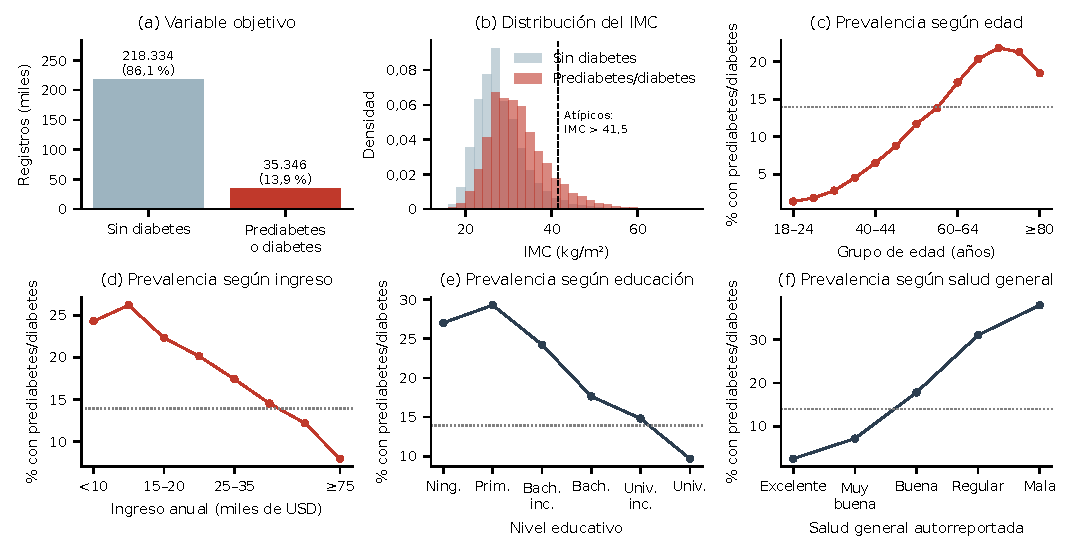
\includegraphics[width=\textwidth]{fig_eda.pdf}
\caption{Análisis exploratorio. (a) Distribución de la variable objetivo. (b) Distribución del IMC por clase; la línea discontinua marca el umbral de valores atípicos (Q3 + 1,5 RIC). (c)--(f) Porcentaje de personas con prediabetes o diabetes según edad, ingreso, educación y salud general; la línea punteada es la prevalencia global.}
\label{fig:eda}
\end{figure*}

\begin{figure}[!t]
\centering
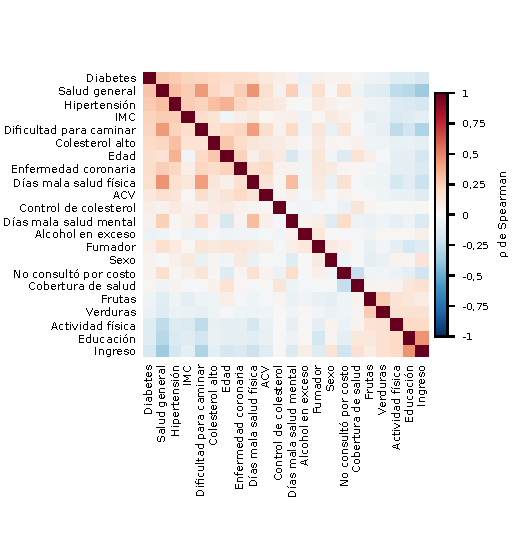
\includegraphics[width=\columnwidth]{fig_correlacion.pdf}
\caption{Correlación de Spearman entre la variable objetivo y las 21 predictoras.}
\label{fig:corr}
\end{figure}

%=====================================================================
\section{Estado del arte}
Se revisaron cinco artículos de revista que abordan el mismo problema de aprendizaje: clasificar a una persona según tenga o no diabetes (o prediabetes) a partir de variables clínicas y de estilo de vida. Dos usan exactamente la misma base de este trabajo~\cite{ren2024,majcherek2025}, uno la encuesta BRFSS de 2014~\cite{xie2019} y dos usan otras fuentes, con información de laboratorio~\cite{dinh2019,zou2018}. Todos usan aprendizaje supervisado de clasificación binaria. La Tabla~\ref{tab:sota} resume la técnica, la validación, las métricas y los resultados de cada uno.

\begin{table*}[!t]
\caption{Trabajos relacionados: todos usan aprendizaje supervisado de clasificación binaria}
\label{tab:sota}
\centering
\footnotesize
\begin{tabular}{L{1.75cm} L{2.75cm} L{3.0cm} L{3.1cm} L{2.05cm} L{4.2cm}}
\toprule
Trabajo & Datos & Técnicas & Validación & Métricas & Resultados \\
\midrule
Xie et al.~\cite{xie2019} (2019) & BRFSS 2014: 138.146 adultos, 27 variables; objetivo: diabetes tipo 2 & SVM (lineal, polinomial, RBF), árbol, regresión logística, Random Forest, red neuronal, Naive Bayes & Partición 2/3 entrenamiento, 1/3 prueba; SMOTE en entrenamiento & AUC, exactitud, sensibilidad, especificidad & Red neuronal: AUC 0,795, exactitud 82,4~\%, sensibilidad 37,8~\%. La mayor sensibilidad (árbol) fue 51,6~\% \\
Dinh et al.~\cite{dinh2019} (2019) & NHANES 1999--2014; 123 variables, con y sin laboratorio & Regresión logística, SVM, Random Forest, XGBoost y ensamble ponderado & Búsqueda en rejilla y validación cruzada de 10 pliegues & AUC, precisión, \emph{recall}, F1 & Diabetes sin laboratorio: XGBoost, AUC 0,862; prediabetes: ensamble, AUC 0,737 (0,844 con laboratorio) \\
Zou et al.~\cite{zou2018} (2018) & Exámenes médicos de un hospital de Luzhou (China), 14 atributos con glucosa en ayunas & Árbol de decisión, Random Forest, red neuronal; PCA y mRMR & Validación cruzada de 5 pliegues sobre 5 submuestras balanceadas y prueba independiente & Exactitud, sensibilidad, especificidad, MCC & Random Forest con todas las variables: exactitud 0,808 \\
Ren~\cite{ren2024} (2024) & \textbf{Esta misma base} (BRFSS 2015, 253.680 registros) & Naive Bayes, árbol, Random Forest, regresión logística, \emph{gradient boosting}, LDA, CatBoost; selección por $\chi^2$ & Partición 80/20; SMOTE en entrenamiento & Exactitud, precisión, ECM & CatBoost en prueba: exactitud 86,6~\%, precisión 55,6~\% \\
Majcherek et al.~\cite{majcherek2025} (2025) & \textbf{Esta misma base} (BRFSS 2015, 253.680 registros) & 18 modelos (Extra Trees, AdaBoost, CatBoost, LightGBM, etc.); SHAP & Partición 80/20 y validación cruzada estratificada; ROS, SMOTE y ADASYN & Exactitud, precisión, \emph{recall}, F1, AUC & Extra Trees: exactitud $>$ 90~\%, AUC 0,99 \\
\bottomrule
\end{tabular}
\end{table*}

Tres observaciones orientan este proyecto. Primero, con datos de encuesta y sin laboratorio, el AUC se ubica entre 0,72 y 0,86~\cite{xie2019,dinh2019}, y la prediabetes es más difícil de separar que la diabetes~\cite{dinh2019}. Segundo, reportar solo la exactitud oculta el problema del desbalance: en Xie et al. la red neuronal tiene la mejor exactitud pero detecta solo el 37,8~\% de los casos, y en Ren la precisión de 55,6~\% contrasta con una exactitud de 86,6~\%. Tercero, Majcherek et al. aplican el sobremuestreo antes de describir la partición, lo que puede dejar muestras sintéticas emparentadas en entrenamiento y prueba; eso explicaría un AUC de 0,99, muy por encima del resto. Por eso aquí la prueba se separa antes de cualquier remuestreo y se reportan métricas adecuadas al desbalance~\cite{he2009,saito2015}. Ninguno de los trabajos cuantifica por separado el aporte de los determinantes sociales y de los factores clínicos.

\textbf{Métrica no vista en clase.} Zou et al. usan el coeficiente de correlación de Matthews, que resume la matriz de confusión en un valor entre $-1$ y $1$ (1 = predicción perfecta, 0 = azar):
\begin{equation}
\mathrm{MCC}=\frac{VP\cdot VN-FP\cdot FN}{\sqrt{D}},
\end{equation}
con $D=(VP+FP)(VP+FN)(VN+FP)(VN+FN)$, donde $VP$, $VN$, $FP$ y $FN$ son los verdaderos y falsos positivos y negativos. Las demás métricas se vieron en clase o se definen en la Sección~\ref{sec:metricas}.

%=====================================================================
\section{Entrenamiento y evaluación de modelos}
\subsection{Configuración experimental}
\textbf{Metodología de validación.} Se separó el 20~\% de la base como conjunto de prueba, de forma estratificada para conservar la prevalencia real (\nPrueba{} registros). Ese conjunto no interviene en ninguna decisión de modelado. Los hiperparámetros se eligieron con búsqueda en malla y validación cruzada estratificada de cinco pliegues, maximizando el AUC-ROC promedio. La estandarización forma parte del \emph{pipeline} de cada modelo, de modo que se ajusta solo con los datos de entrenamiento de cada pliegue y no hay fuga de información hacia la validación.

\textbf{Submuestreo.} Del 80~\% restante (\nPool{} registros) se extrajo una muestra de entrenamiento balanceada de \nEntrenamiento{} registros, 10.000 de cada clase, mediante submuestreo aleatorio sin reemplazo de la clase mayoritaria. El submuestreo se hace después de separar la prueba, así que esta conserva la distribución real. La decisión atiende dos problemas: el desbalance y el costo de SVM y KNN, que crece de forma superlineal con el número de muestras. Para verificar que no se pierde información, se entrenó además una regresión logística con los \controlN{} registros y pesos por clase (Sección~\ref{sec:resultados}).

\subsection{Modelos e hiperparámetros}
Se comparan los cinco tipos de modelo que pide la guía. La Tabla~\ref{tab:malla} muestra la malla de hiperparámetros explorada en cada uno y la configuración elegida. Los modelos se implementaron con scikit-learn~\cite{pedregosa2011}.

\begin{table*}[!t]
\caption{Modelos comparados, malla de hiperparámetros explorada y configuración elegida por validación cruzada}
\label{tab:malla}
\centering
\footnotesize
\begin{tabular}{L{3.0cm} L{2.2cm} L{7.4cm} L{3.7cm}}
\toprule
Tipo & Modelo & Hiperparámetros y malla de valores & Configuración elegida \\
\midrule
\inputtabla{generado/tabla_malla.tex}
\bottomrule
\end{tabular}
\end{table*}

\subsection{Métricas de desempeño}\label{sec:metricas}
El AUC-ROC es el criterio de selección porque no depende de un umbral de decisión ni de la prevalencia. Como complemento se reportan la sensibilidad (proporción de casos detectados, la más importante en tamizaje), la especificidad, la precisión y el F1, vistas en clase, y dos métricas que no se vieron en clase y que son apropiadas para clases desbalanceadas:

\textbf{Exactitud balanceada}, el promedio de sensibilidad y especificidad; a diferencia de la exactitud, un modelo que siempre prediga la clase mayoritaria obtiene 0,5:
\begin{equation}
\mathrm{EB}=\frac{1}{2}\left(\frac{VP}{VP+FN}+\frac{VN}{VN+FP}\right).
\end{equation}

\textbf{AUC-PR}, el área bajo la curva de precisión y sensibilidad, estimada como la precisión promedio sobre los umbrales $n$ ordenados del puntaje:
\begin{equation}
\mathrm{AUC\text{-}PR}=\sum_{n}\left(R_n-R_{n-1}\right)P_n,
\end{equation}
donde $P_n$ y $R_n$ son la precisión y la sensibilidad en el umbral $n$. A diferencia del AUC-ROC, depende de la prevalencia: \textbf{un clasificador aleatorio obtiene un AUC-PR igual a la prevalencia} (\lineaBasePR{} en la prueba), y esa es la línea base para interpretarla~\cite{saito2015}.

Las métricas de entrenamiento y validación se reportan como media $\pm$ desviación estándar en los cinco pliegues. Las de prueba incluyen un intervalo de confianza del 95~\% por \emph{bootstrap} (500 remuestreos del conjunto de prueba). El umbral de decisión es 0,5, que en una muestra balanceada equivale a no favorecer ninguna clase.

\subsection{Resultados}\label{sec:resultados}
\textbf{Efecto de los hiperparámetros.} La Fig.~\ref{fig:hiper} muestra el AUC-ROC de entrenamiento y de validación en toda la malla. En KNN, con pocos vecinos el modelo memoriza (AUC de entrenamiento de 1 con pesos por distancia) y la validación cae a 0,77; desde unos 50 vecinos se estabiliza en 0,81. En Random Forest, los árboles sin límite de profundidad y con una muestra por hoja también memorizan (entrenamiento 1,000, validación 0,814); exigir 10 muestras por hoja reduce esa brecha y sube la validación a 0,826. En el perceptrón multicapa, la regularización más fuerte ($\alpha$ = 1) da el mejor resultado. En la SVM, $\gamma$ = escala con $C$ = 10 sobreajusta, mientras que $\gamma$ = 0,01 es estable. La regresión logística es insensible a $C$ desde 0,01.

\begin{figure*}[!t]
\centering
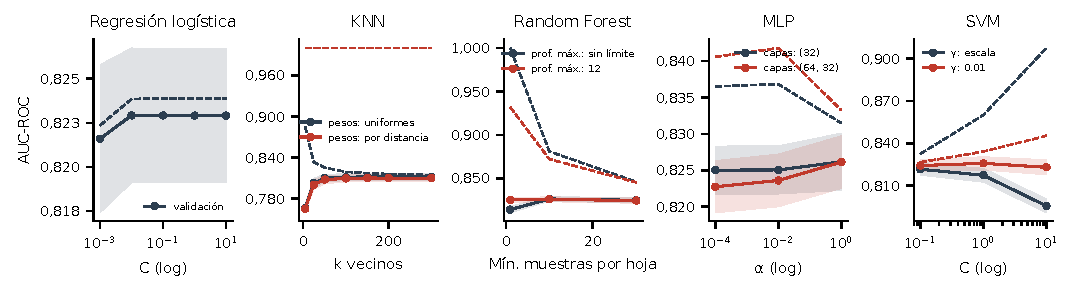
\includegraphics[width=\textwidth]{fig_hiperparametros.pdf}
\caption{Efecto de los hiperparámetros: AUC-ROC promedio de validación (línea continua, banda de $\pm$ una desviación estándar) y de entrenamiento (línea discontinua) en la validación cruzada de cinco pliegues.}
\label{fig:hiper}
\end{figure*}

\textbf{Entrenamiento, validación y prueba.} La Tabla~\ref{tab:resultados} reporta todas las métricas en las tres fases. El AUC de prueba queda entre \pruebaAucKNN{} (KNN) y \pruebaAucMLP{} (perceptrón multicapa), siempre dentro de una centésima del de validación, lo que indica que la selección de hiperparámetros no sobreajustó. Random Forest es el único con una brecha notable entre entrenamiento (\entAucRF) y validación (\valAucRF). Los intervalos de confianza de los cuatro mejores modelos se traslapan, así que sus diferencias no son significativas; KNN es el más débil, algo esperable en un modelo de distancias cuando 14 de las 21 variables son binarias.

\begin{table*}[!t]
\caption{Desempeño de los cinco modelos con la configuración elegida. Entrenamiento y validación: media $\pm$ desviación estándar en los cinco pliegues de la validación cruzada. Prueba: \nPrueba{} registros con la prevalencia real, con intervalo de confianza del 95~\% por \emph{bootstrap}. Umbral de decisión: 0,5.}
\label{tab:resultados}
\centering
\footnotesize
\setlength{\tabcolsep}{3.5pt}
\begin{tabular}{l l c c c c c c}
\toprule
Modelo & Fase & AUC-ROC & AUC-PR & Sensibilidad & Especificidad & F1 & Exactitud balanceada \\
\midrule
\inputtabla{generado/tabla_resultados.tex}
\bottomrule
\end{tabular}
\end{table*}

La Fig.~\ref{fig:curvas} muestra las curvas ROC y de precisión--sensibilidad en prueba. En la muestra balanceada el AUC-PR de validación ronda 0,8, pero en prueba cae a 0,38--0,41 porque allí la prevalencia es \prevalencia{}. Frente a la línea base de \lineaBasePR{}, los modelos multiplican por casi tres la precisión de una clasificación al azar. La precisión en prueba ronda el 30~\%: de cada diez personas señaladas, tres tienen la condición. Es el costo de una sensibilidad cercana al 80~\% en una población con pocos casos, aceptable para tamizaje, cuyo propósito es decidir a quién remitir a una prueba de laboratorio. Para verificar que el submuestreo no resta información, una regresión logística entrenada con los \controlN{} registros y pesos por clase obtuvo un AUC de prueba de \controlAuc, frente a \pruebaAucLR{} con la muestra balanceada.

\begin{figure*}[!t]
\centering
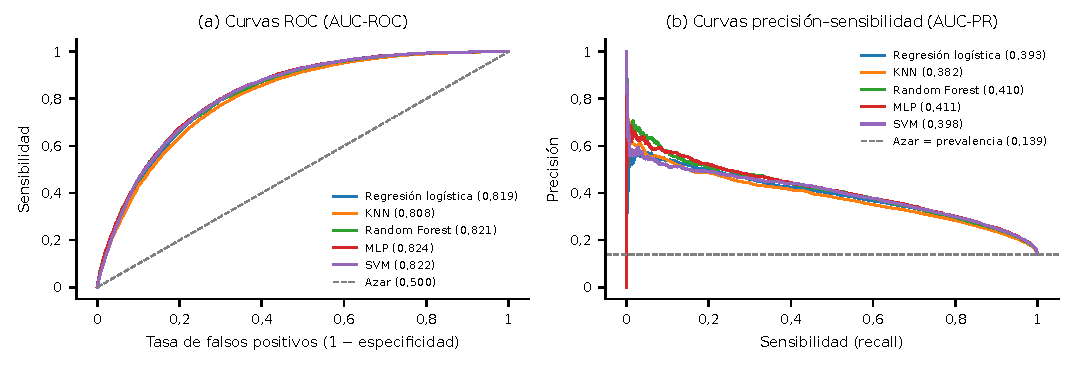
\includegraphics[width=\textwidth]{fig_curvas.pdf}
\caption{Curvas en el conjunto de prueba. (a) ROC; entre paréntesis, el AUC-ROC. (b) Precisión--sensibilidad; entre paréntesis, el AUC-PR. La línea discontinua de (b) es la prevalencia, que equivale al AUC-PR de un clasificador aleatorio.}
\label{fig:curvas}
\end{figure*}

\textbf{Determinantes sociales frente a factores clínicos.} La Tabla~\ref{tab:bloques} compara modelos entrenados con cada bloque de variables. Las diez variables clínicas alcanzan solas un AUC de \bloqueRfClinico, muy cerca del modelo completo (\bloqueRfTodas). Las cuatro variables socioeconómicas y de acceso obtienen \bloqueRfSocial, y sumadas a la edad y el sexo llegan a \bloqueRfSocialDemo: discriminan claramente mejor que el azar, pero su aporte adicional es pequeño una vez se conocen las variables clínicas. Una lectura compatible con los datos es que su efecto se manifiesta a través de factores como la obesidad y la hipertensión; al tratarse de una encuesta transversal, el análisis no permite afirmar causalidad.

\begin{table}[!t]
\caption{AUC-ROC en prueba según el bloque de variables}
\label{tab:bloques}
\centering
\footnotesize
\begin{tabular}{l c c c}
\toprule
Bloque & Variables & Reg. logística & Random Forest \\
\midrule
\inputtabla{generado/tabla_bloques.tex}
\bottomrule
\end{tabular}
\end{table}

%=====================================================================
\section{Reducción de dimensión}
\begin{figure}[!t]
\centering
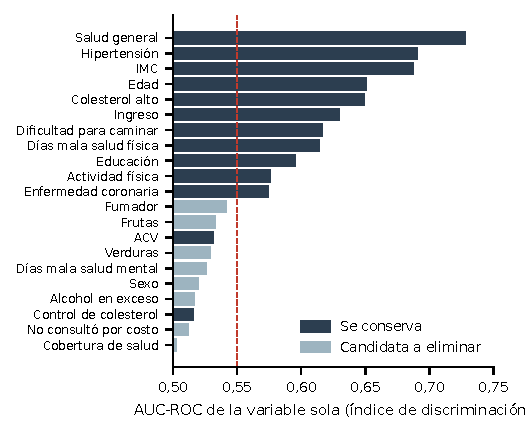
\includegraphics[width=\columnwidth]{fig_individual.pdf}
\caption{Índice de discriminación de cada variable: AUC-ROC obtenido con la variable sola. La línea discontinua marca el umbral de 0,55; en gris, las candidatas a eliminar.}
\label{fig:individual}
\end{figure}
\begin{figure*}[!t]
\centering
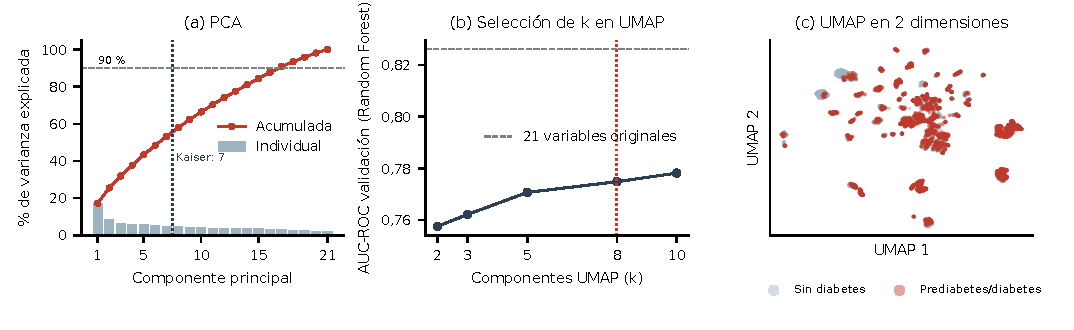
\includegraphics[width=\textwidth]{fig_reduccion.pdf}
\caption{(a) PCA: varianza explicada por componente y acumulada; la línea punteada marca el criterio de Kaiser y la discontinua el 90~\%. (b) UMAP: AUC-ROC en la partición de validación según el número de componentes; la línea punteada marca el $k$ elegido y la discontinua, el AUC de validación cruzada con las 21 variables originales. (c) Proyección UMAP en dos dimensiones de una muestra de 6.000 registros de entrenamiento.}
\label{fig:reduccion}
\end{figure*}

\begin{table*}[!t]
\caption{Reducción de dimensión con los dos mejores modelos. Validación: AUC-ROC media $\pm$ desviación estándar en cinco pliegues ($\dagger$: partición de validación 80/20 usada para elegir $k$). Prueba: AUC-ROC con intervalo de confianza del 95~\%, AUC-PR y exactitud balanceada (EB).}
\label{tab:reduccion}
\centering
\footnotesize
\begin{tabular}{l c c l c c c c}
\toprule
Representación & Dim. & Reducción & Modelo & AUC validación & AUC prueba (IC 95~\%) & AUC-PR & EB \\
\midrule
\inputtabla{generado/tabla_reduccion.tex}
\bottomrule
\end{tabular}
\end{table*}

Se evalúa si es posible reducir la complejidad del modelo con tres técnicas: selección de variables a partir de un análisis individual, extracción lineal con PCA y extracción no lineal con UMAP. Como pide la guía, cada representación se prueba con los dos mejores modelos de la Sección~IV, elegidos por su AUC de \emph{validación} y no de prueba para no contaminar la selección: \mejorUno{} y \mejorDos{}, prácticamente empatados (\valAucRF{} y \valAucMLP). Las transformaciones se ajustan dentro de cada pliegue de la validación cruzada. La Tabla~\ref{tab:reduccion} reúne los resultados.

\subsection{Análisis individual de variables}
Para cada variable se calcularon tres medidas de su relación con la clase en la muestra de entrenamiento: la correlación de Spearman, la información mutua y un índice de discriminación, que es el AUC-ROC obtenido al usar la variable sola como puntaje (Fig.~\ref{fig:individual}). La salud general, la hipertensión, el IMC, la edad y el colesterol alto son las más discriminativas.

Se consideran \textbf{candidatas a eliminar} las variables que discriminan casi como el azar (AUC individual menor que 0,55) y además comparten muy poca información con la clase ($|\rho| < 0{,}10$): fumador, consumo de frutas, consumo de verduras, días de mala salud mental, sexo, consumo excesivo de alcohol, no consultar por costo y cobertura de salud. El ACV y el control de colesterol tienen un AUC individual bajo porque son poco frecuentes, pero su correlación con la clase supera el umbral, así que se conservan. Al retirar las \nCandidatas{} candidatas quedan \nConservadas{} variables (\selRed{} de reducción) y el AUC de prueba baja menos de cinco milésimas en ambos modelos.



\subsection{Extracción lineal: PCA}
PCA se aplicó a las variables estandarizadas. La primera componente explica solo el \pcaPcUno{} de la varianza y combina salud general, dificultad para caminar y días de mala salud física con signo opuesto al ingreso y la educación: un eje de deterioro de la salud asociado a la desventaja socioeconómica.

\textbf{Criterio para el número de componentes.} Se compararon dos criterios estándar. El de Kaiser conserva las componentes con autovalor mayor que 1, es decir, las que explican más varianza que una variable original estandarizada: son \pcaKaiser{} componentes, que retienen el \pcaVarKaiser{} de la varianza (\pcaRedKaiser{} de reducción). El del 90~\% de varianza explicada requiere \pcaNoventa{} componentes (\pcaRedNoventa{} de reducción), porque las variables están poco correlacionadas entre sí (Fig.~\ref{fig:reduccion}a). Se elige el criterio de Kaiser: con un tercio de las dimensiones pierde alrededor de una centésima de AUC, mientras que el del 90~\% casi no reduce la dimensión y en Random Forest no mejora el resultado.

\subsection{Extracción no lineal: UMAP}
UMAP~\cite{mcinnes2018} construye un grafo de vecinos y busca una proyección de baja dimensión que preserve la estructura local; se usaron 30 vecinos y distancia mínima 0. \textbf{Criterio.} Como UMAP no tiene una medida de varianza explicada, el número de componentes se eligió por desempeño: se probaron $k \in \{2, 3, 5, 8, 10\}$ en una partición de validación (80/20) de la muestra de entrenamiento con \mejorUno, y se escogió el menor $k$ cuyo AUC quedara a menos de 0,005 del máximo (Fig.~\ref{fig:reduccion}b): $k$ = \umapK{} (\umapRed{} de reducción). Aun así, el AUC de prueba cae a 0,77 con Random Forest y a 0,74 con el perceptrón. La proyección en dos dimensiones (Fig.~\ref{fig:reduccion}c) muestra la causa: los vecindarios se forman por combinaciones repetidas de respuestas binarias, no por la condición de salud, y las dos clases quedan mezcladas dentro de cada grupo.



%=====================================================================
\section{Discusión y conclusiones}
\textbf{Desempeño.} Con indicadores autorreportados es posible detectar prediabetes o diabetes con un AUC-ROC de prueba de hasta \pruebaAucMLP{} y una sensibilidad cercana al 80~\%. El resultado supera el rango de 0,72--0,80 de Xie et al.~\cite{xie2019} con la encuesta de 2014, aunque su objetivo era solo la diabetes tipo 2, y es comparable con el 0,862 de Dinh et al.~\cite{dinh2019} para diabetes sin laboratorio, que usaron 123 variables. La mejora frente a trabajos que reportan sensibilidades del 38 al 52~\% se explica más por el tratamiento del desbalance que por el algoritmo: los cuatro mejores modelos quedan dentro del margen de variación de la validación cruzada. El AUC de 0,99 que reportan Majcherek et al.~\cite{majcherek2025} con la misma base no es comparable, por el orden en que aplican el sobremuestreo.

\textbf{Determinantes sociales.} La capacidad predictiva proviene sobre todo de las variables clínicas. Los determinantes sociales discriminan por sí solos y muestran un gradiente claro de prevalencia, pero aportan poco una vez se conocen los factores clínicos.

\textbf{Reducción de dimensión.} Sí es posible reducir la complejidad del modelo final: la selección de variables retira el \selRed{} de las variables casi sin pérdida, porque elimina directamente las que no discriminan. PCA, con el criterio de Kaiser, reduce a \pcaKaiser{} componentes a costa de una centésima de AUC, ya que maximiza la varianza sin mirar la clase y las variables están poco correlacionadas. UMAP es la peor opción para este problema, porque su noción de vecindad no coincide con la separación entre clases. Para un modelo final se recomienda la selección de variables, que además conserva la interpretabilidad.

\textbf{Limitaciones.} (i) Todas las variables, incluida la etiqueta, son autorreportadas, así que hay sesgo de memoria y de deseabilidad social, y la etiqueta no incluye la diabetes no diagnosticada, que es justamente la que el tamizaje busca. (ii) La etiqueta agrupa prediabetes y diabetes, dos condiciones con perfiles distintos. (iii) Es una encuesta transversal: las asociaciones no son causales. (iv) No se usaron los pesos muestrales del BRFSS, por lo que las prevalencias describen la muestra y no la población de Estados Unidos. (v) Los resultados corresponden a la población estadounidense de 2015 y no se pueden trasladar directamente a Colombia.

\textbf{Trabajo futuro.} Ajustar el umbral de decisión según el costo de los falsos negativos, calibrar las probabilidades y evaluar el desempeño por subgrupos de ingreso y educación, para verificar que el modelo no detecta peor a las poblaciones con mayor prevalencia.

\bibliographystyle{IEEEtran}
\bibliography{referencias}

\end{document}
